% move all configuration stuff into one file so we can focus on the content
\documentclass[aspectratio=169,hyperref={pdfpagelabels=false,colorlinks=true,linkcolor=white,urlcolor=blue},t]{beamer}

%%%%%%%%%%%%%%%%%%%%%%%%%%%%%%%%%%%%%%%%%%%%%%%%%%%%%%%%%%%%%%%%%%%%%%%%%%%%%%%%%%
%%%%%%%%%%%%%%%%%%%%%%%%%%%%%%%%%%%%%%%%%%%%%%%%%%%%%%%%%%%%%%%%%%%%%%%%%%%%%%%%%%
% packages
\usepackage{pict2e}
\usepackage{epic}
\usepackage{amsmath,amsfonts,amssymb}
\usepackage{units}
\usepackage{fancybox}
\usepackage[absolute,overlay]{textpos} 
\usepackage{media9} % avi2flv: "C:\Program Files\ffmpeg\bin\ffmpeg.exe" -i TuneFreqFilterbank.avi -b 600k -s 441x324 -r 15 -acodec copy TuneFreqFilterbank.flv
\usepackage{animate}
\usepackage{gensymb}
\usepackage{multirow}
\usepackage{silence}
\usepackage[backend=bibtex,style=ieee]{biblatex}
\AtEveryCitekey{\iffootnote{\tiny}{}}
\addbibresource{references}

%%%%%%%%%%%%%%%%%%%%%%%%%%%%%%%%%%%%%%%%%%%%%%%%%%%%%%%%%%%%%%%%%%%%%%%%%%%%%%%%%%
%%%%%%%%%%%%%%%%%%%%%%%%%%%%%%%%%%%%%%%%%%%%%%%%%%%%%%%%%%%%%%%%%%%%%%%%%%%%%%%%%%
% relative paths
\graphicspath{{graph/}}


%%%%%%%%%%%%%%%%%%%%%%%%%%%%%%%%%%%%%%%%%%%%%%%%%%%%%%%%%%%%%%%%%%%%%%%%%%%%%%%%%%
%%%%%%%%%%%%%%%%%%%%%%%%%%%%%%%%%%%%%%%%%%%%%%%%%%%%%%%%%%%%%%%%%%%%%%%%%%%%%%%%%%
% units
\setlength{\unitlength}{1mm}

%%%%%%%%%%%%%%%%%%%%%%%%%%%%%%%%%%%%%%%%%%%%%%%%%%%%%%%%%%%%%%%%%%%%%%%%%%%%%%%%%%
%%%%%%%%%%%%%%%%%%%%%%%%%%%%%%%%%%%%%%%%%%%%%%%%%%%%%%%%%%%%%%%%%%%%%%%%%%%%%%%%%%
% theme & layout
\usetheme{Frankfurt}
\beamertemplatenavigationsymbolsempty
%\setbeamertemplate{frametitle}[smoothbars theme]
\setbeamertemplate{frametitle}
{
    \begin{beamercolorbox}[ht=1.8em,wd=\paperwidth]{frametitle}
        \vspace{-.1em}%
        \hspace{.2em}{\strut\insertframetitle\strut}
        
        \hspace{.2em}\small\strut\insertframesubtitle\strut
        %\hfill
        %
\includegraphics[height=.8cm,keepaspectratio]{CenterMusicTechnology-solid-2lines-white-CoAtag}
        
    \end{beamercolorbox}
    \begin{textblock*}{100mm}(11.6cm,.7cm)
        \includegraphics[height=.8cm,keepaspectratio]{logo_GTCMT_black}
    \end{textblock*}
}

% set this to ensure bulletpoints without subsections
\usepackage{remreset}
\makeatletter
\@removefromreset{subsection}{section}
\makeatother
\setcounter{subsection}{1}

%---------------------------------------------------------------------------------
% appearance
\setbeamercolor{structure}{fg=gtgold}
\setbeamercovered{transparent} %invisible
\setbeamercolor{bibliography entry author}{fg=black}
\setbeamercolor*{bibliography entry title}{fg=black}
\setbeamercolor*{bibliography entry note}{fg=black}

%\usepackage{pgfpages}
%\setbeameroption{show notes}
%\setbeameroption{show notes on second screen=right}
%---------------------------------------------------------------------------------
% fontsize
\let\Tiny=\tiny

%%%%%%%%%%%%%%%%%%%%%%%%%%%%%%%%%%%%%%%%%%%%%%%%%%%%%%%%%%%%%%%%%%%%%%%%%%%%%%%%%%
%%%%%%%%%%%%%%%%%%%%%%%%%%%%%%%%%%%%%%%%%%%%%%%%%%%%%%%%%%%%%%%%%%%%%%%%%%%%%%%%%%
% warnings
\pdfsuppresswarningpagegroup=1
\WarningFilter{biblatex}{Patching footnotes failed}
\WarningFilter{latexfont}{Font shape}
\WarningFilter{latexfont}{Some font shapes}
\WarningFilter{gensymb}{Not defining}



\subtitle{Part 7.1: Temporal Analysis}

%%%%%%%%%%%%%%%%%%%%%%%%%%%%%%%%%%%%%%%%%%%%%%%%%%%%%%%%%%%%%%%%%%%%%%%%%%%%
\begin{document}
    % generate title page
	

\begin{frame}
    \titlepage
    %\vspace{-5mm}
    \begin{flushright}
        \href{http://www.gtcmt.gatech.edu}{\includegraphics[height=.8cm,keepaspectratio]{logo_GTCMT_black}}
    \end{flushright}
\end{frame}


    \section[overview]{lecture overview}
        \begin{frame}{temporal analysis}{overview}
            \begin{itemize}
                \item   \textbf{text book}  
                    \begin{itemize}
                        \item   \href{http://ieeexplore.ieee.org/xpl/articleDetails.jsp?tp=&arnumber=6331123&}{\underline{\textit{Chapter 6: Temporal Analysis} (pp.~119--136)}}
                    \end{itemize}
                \bigskip
                \item<2->   \textbf{lecture content}
                    \begin{itemize}
                        \item<2->   human perception of temporal events
                        \item<3->   temporal events in music
                        \item<4->   onset detection
                        \item<5->   tempo detection
                    \end{itemize}
            \end{itemize}
        \end{frame}

    \section[intro]{introduction}
        \begin{frame}{temporal events}{introduction}
            \begin{itemize}
                \item  \textbf{categorization of temporal parameters}:
                    \begin{itemize}
                        \item	\textit{score} parameters:\\ structure, time signature, rhythm, \ldots
                        \item	\textit{performance} parameters:\\ tempo, timing, \ldots
                    \end{itemize}
                \bigskip
                \item<2->   \textbf{perception of temporal parameters}:
                    \begin{itemize}
                        \item	audio signal/stream is segmented into distinct events $\Rightarrow$ \textit{onsets} (segment start)
                        \item	humans \textit{structure and group} these events due to position, salience, \ldots
                    \end{itemize}
            \end{itemize}
        \end{frame}

    \section[perception]{human perception of temporal events}
        \begin{frame}{human perception of temporal events}{onsets 1/3}
            \begin{itemize}
                \item   \textbf{definition}: onset is start of a musical event
                \item<2->   \textbf{properties}:
                    \begin{itemize}
                        \item<3->	position
                        \item<3->	strength, salience
                        \item<3->	length?
                    \end{itemize}
            \end{itemize}
                \only<3->{\figwithmatlab{Onset}}
        \end{frame}

        \begin{frame}{human perception of temporal events}{onsets 2/3}
            \question{typical initial transient lengths}
            \begin{itemize}
                \item	percussive instrument:\\ \unit[3-20]{ms}
                \item	woodwind instrument:\\ up to \unit[300]{ms}
                \item	typical range:\\ \unit[15-50]{ms}
            \end{itemize}
        \end{frame}
        \begin{frame}{human perception of temporal events}{onsets 3/3}
            \begin{itemize}
                \item	\textit{detection \& discrimination} of 2 subsequent onsets
                    \begin{itemize}
                        \item	detection $\Delta t > \unit[2]{ms}$, discrimination $\Delta t > \unit[20]{ms}$\only<1>{\footfullcite{hirsh_auditory_1959}}
                    \end{itemize}
                
                \item<2->	\textit{prediction} of looped monophonic instrument onsets
                    \begin{itemize}
                        \item	IOI \unit[600]{ms}: $\sigma = \unit[12]{ms}$\only<2>{\footfullcite{gordon_perception_1984}}
                        \item	IOI $<$ \unit[240]{ms}: $\sigma = \unit[10]{ms}$\only<2>{\footfullcite{friberg_perception_1992}}
                    \end{itemize}

                \item<3->	manual onset time \textit{annotation}
                    \begin{itemize}
                        \item	piano: mean abs.\ error: \unit[4.3]{ms}, max: \unit[35]{ms}\only<3>{\footfullcite{repp_diversity_1992}}
                        \item	various: mean abs.\ error: \unit[10]{ms}, max: \unit[30]{ms}\only<3>{\footfullcite{leveau_methodology_2004}}
                    \end{itemize}
                
                \item<4->	ensemble performance
                    \begin{itemize}
                        \item	string \& woodwind: deviations up to  \unit[30-50]{ms}\only<4>{\footfullcite{rasch_synchronization_1979}}
                        \item	piano: $\sigma = \unit[14-38]{ms}$\only<4>{\footfullcite{shaffer_timing_1984}}
                    \end{itemize}
            \end{itemize}
        \end{frame}

        \begin{frame}{human perception of temporal events}{offsets}
            \question{what about offsets/end of notes}

            \begin{itemize}
                \item   \textbf{perceptually not as important} as an onset
                    \begin{itemize}
                        \item   offset are often ignored in rhythm perception
                    \end{itemize}
                \smallskip
                \item<2->	\textbf{systematic difficulties}: when does a note end?
                    \begin{itemize}
                        \item	performer stops excitation
                        \item	instrument stops oscillation
                        \item	listener cannot recognize it anymore
                    \end{itemize}
                \smallskip
                \item<3->	\textbf{practical difficulties}: hard to detect
                    \begin{itemize}
                        \item	low volume
                        \item	reverberation
                        \item	masking
                    \end{itemize}
            \end{itemize}
        \end{frame}
        
        \begin{frame}{human perception of temporal events}{tempo, meter \& rhythm}
            \begin{itemize}
                \item	\textbf{tempo}
                    \begin{itemize}
                        \item<2->	perceived equal duration pulses at a ``natural'' rate: tactus
                        
                        \item<3->	constant tempo
                            \begin{footnotesize}
                            \begin{equation*}\label{eq:tempo_mean}
                                \mathfrak{T} = \frac{ \mathcal{B}\cdot \unit[60]{s}}{\Delta t_\mathrm{s}}\;\; [\unit{BPM}] 
                            \end{equation*}
                            \end{footnotesize}
                        \item<4->	dynamic tempo
                            \begin{footnotesize}
                            \begin{equation*}
                                \mathfrak{T}_\mathrm{local}(j) = \frac{\unit[60]{s}}{t_\mathrm{b}(j+1)-t_\mathrm{b}(j)}\;\; [\unit{BPM}] 
                            \end{equation*}
                            \end{footnotesize}
                            
                            \pause
                            perceived overall tempo?
                            \begin{itemize}
                                \item	average, main, mode, \ldots
                            \end{itemize}
                    \end{itemize}
                \item<6->	\textbf{meter}
                    \begin{itemize}
                        \item	group of strong and weak musical elements/beats
                        \pause
                        \item	typically 3 to 7 beats (app.\ \unit[5]{s})
                    \end{itemize}
                
                \item<7->	\textbf{rhythm}
                    \begin{itemize}
                        \item	group length \unit[1-8]{beats}
                        \item	defined by accents and time intervals
                    \end{itemize}
            \end{itemize}
        \end{frame}

    \section[musical]{musical notation of temporal events}
        \begin{frame}{musical notation of temporal events}{tempo, time signature, bar \& note value}
            \begin{itemize}
                \item	\textbf{tempo}
                    \begin{itemize}
                        \item	\textsl{Largo}, \textsl{Adagio}, \textsl{Andante}, \textsl{Moderato}, \textsl{Allegro}, \textsl{Presto}
                        \pause
                        \item	\textsl{ritardando}, \textsl{accelerando}, \ldots
                        \pause
                        \item	modern scores: indication of overall tempo in \unit{BPM}
                    \end{itemize}
                \smallskip
                \item<2->	\textbf{bar}
                    \begin{itemize}
                        \item	score equivalent of perceptual meter
                        \pause
                        \item	begin of bar is marked by a vertical line
                    \end{itemize}
                \smallskip
                \item<3->	\textbf{time signature}
                    \begin{itemize}
                        \item	conveys length of bar
                            \only<3->{\begin{flushright}
                                \vspace{-10mm}
                                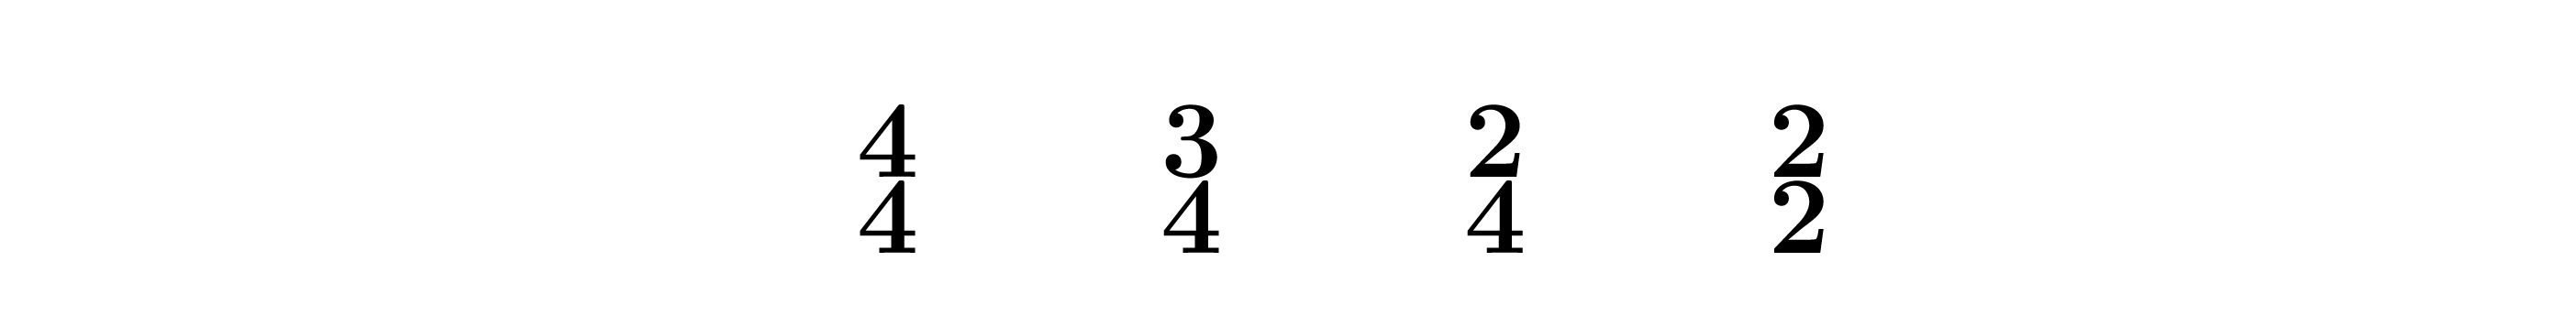
\includegraphics[scale=.5]{onset_timesigs}
                            \end{flushright}}
                    \end{itemize}
                \smallskip
                \item<4->	\textbf{note value}
                            \only<4->{\begin{flushright}
                                \vspace{-5mm}
                                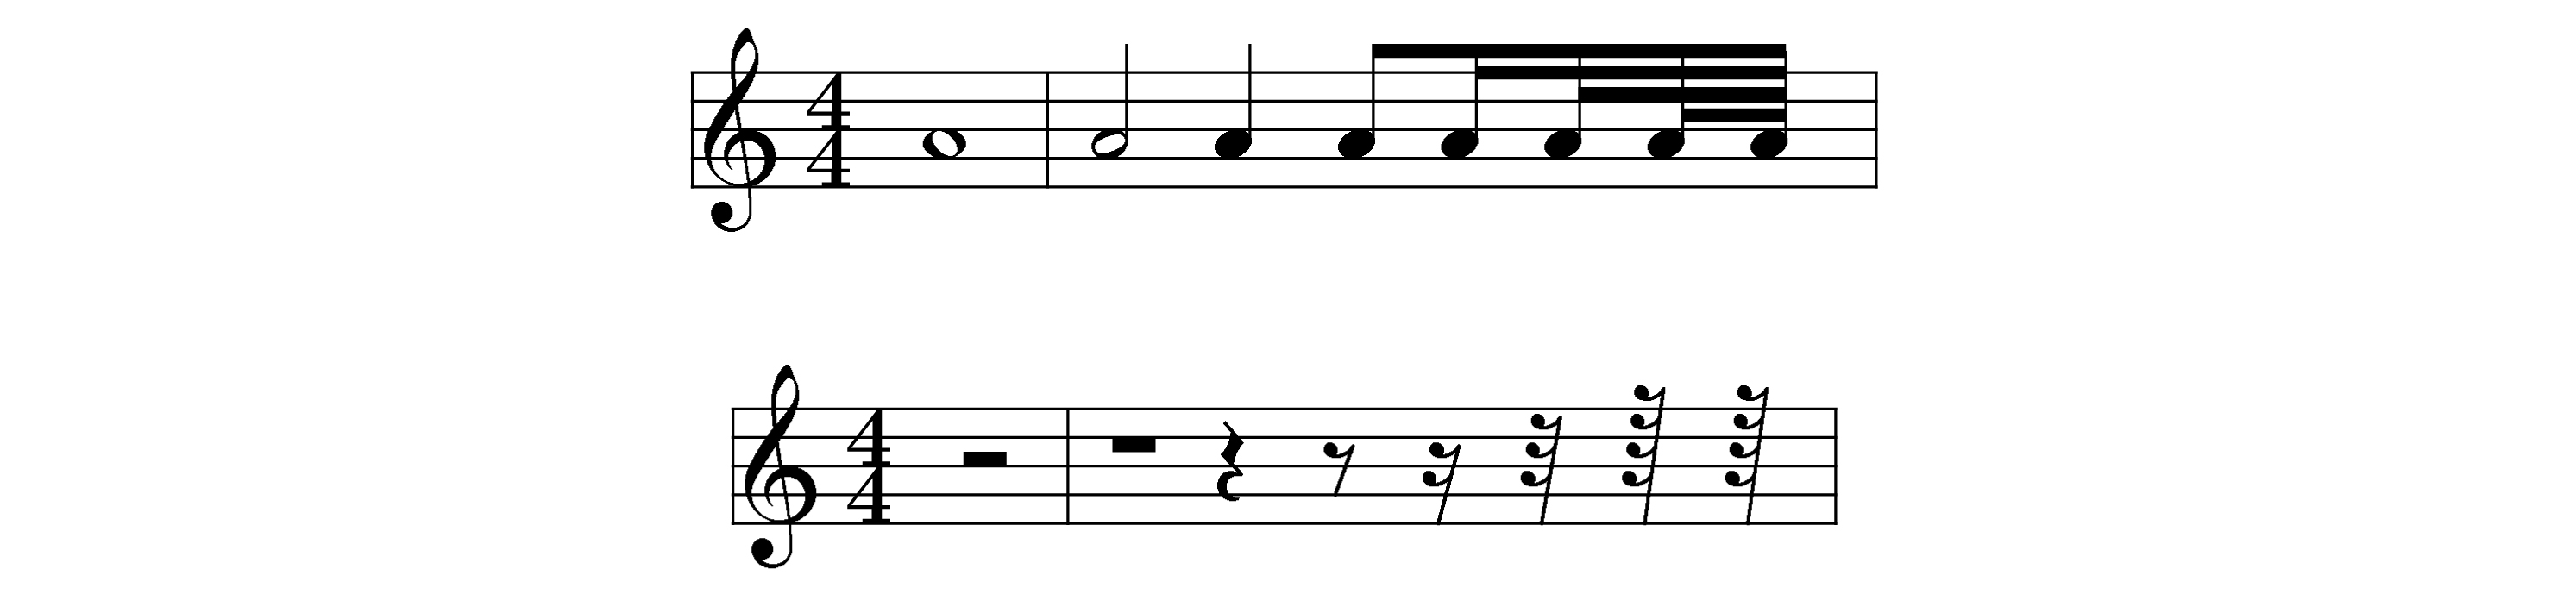
\includegraphics[scale=.6]{onset_notevalues}
                            \end{flushright}}
            \end{itemize}
        \end{frame}
        
    \section[onsets]{onset detection}
        \begin{frame}{onset detection}{brainstorm}
            \question{what are your ideas for detecting the onsets in a complex mixture}
        \end{frame}
        \begin{frame}{onset detection}{introduction}
            \begin{figure}
                \centering
                \begin{footnotesize}
	\begin{picture}(100,26)
		\setcounter{iXOffset}{0}
		\setcounter{iYOffset}{5}
		\setcounter{iXBlockSize}{28}
		\setcounter{iYBlockSize}{16}
		\setcounter{iYBlockSizeDiv2}{8}
		\setcounter{iDistance}{8}

		\put(\value{iXOffset}, 10.5)
			{\text{{\shortstack[c]{Audio\\ Signal}}}}

		\addtocounter{iYOffset}{\value{iYBlockSizeDiv2}}
		\addtocounter{iXOffset}{\value{iDistance}}

		\put(\value{iXOffset}, \value{iYOffset})
			{\vector(1,0){\value{iDistance}}}

		\addtocounter{iXOffset}{\value{iDistance}}
		\addtocounter{iYOffset}{-\value{iYBlockSizeDiv2}}
		
		\put(\value{iXOffset}, \value{iYOffset})
			{\framebox(\value{iXBlockSize}, \value{iYBlockSize}) {{\shortstack[c]{Novelty\\ Function}}}}

		\addtocounter{iXOffset}{\value{iXBlockSize}}
		\addtocounter{iYOffset}{\value{iYBlockSizeDiv2}}

		\put(\value{iXOffset}, \value{iYOffset})
			{\vector(1,0){\value{iDistance}}}

		\addtocounter{iXOffset}{\value{iDistance}}
		\addtocounter{iYOffset}{-\value{iYBlockSizeDiv2}}

		\put(\value{iXOffset}, \value{iYOffset})
			{\framebox(\value{iXBlockSize}, \value{iYBlockSize}) {{\shortstack[c]{Peak\\ Picking}}}}

		\addtocounter{iXOffset}{\value{iXBlockSize}}
		\addtocounter{iYOffset}{\value{iYBlockSizeDiv2}}

		\put(\value{iXOffset}, \value{iYOffset})
			{\vector(1,0){\value{iDistance}}}

		\addtocounter{iXOffset}{\value{iDistance}}
		\addtocounter{iXOffset}{-1}

		%\addtocounter{iYOffset}{-2}
		\put(\value{iXOffset}, 10.5)
			{\text{{\shortstack[c]{Series of\\ Onset Times}}}}
		
	\end{picture}
\end{footnotesize}
            \end{figure}
            
            \begin{itemize}
                \item<2-> 	\textbf{novelty function}
                    \begin{itemize}
                        \item	measure of probability for new events/signal change over time	
                    \end{itemize}
                
                \bigskip
                \item<3->	\textbf{peak picking}
                    \begin{itemize}
                        \item	identify the most likely locations for onsets
                    \end{itemize}
            \end{itemize}
        \end{frame}
        \begin{frame}{onset detection}{novelty function}
            \begin{itemize}
                \item	\textbf{terms}
                    \begin{itemize}
                        \item	detection function
                        \item	difference function
                    \end{itemize}
                \bigskip
                \item<2->	\textbf{extraction}
                    \begin{enumerate}
                        \item<2->	extract features
                        \item<3->	compute derivative
                        \item<4->	smooth result
                        \item<5->	apply $HWR$
                    \end{enumerate}
            \end{itemize}
        \end{frame}
        \begin{frame}{onset detection}{novelty function examples 1/2}
            \begin{enumerate}
                \item	\textbf{time domain}
                    \begin{itemize}
                        \item	extract time domain envelope
                        \item<2->	calculate the slope
                    \end{itemize}
                    \only<1-2>{\figwithmatlab{Onset}}
                \bigskip
                \item<3->	\textbf{pitch-based}: evaluate pitch changes\footfullcite{collins_using_2005}
                        \begin{figure}[t]
                            \centering
                            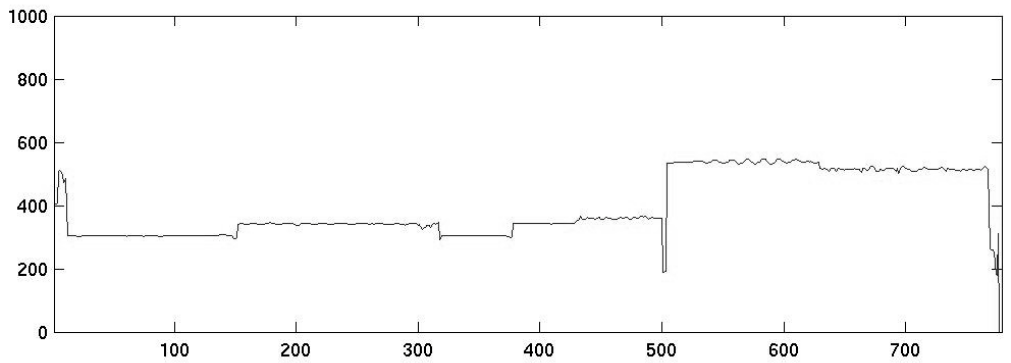
\includegraphics[scale=.25]{graph/pitch_onset}
                        \end{figure}
            \end{enumerate}
        \end{frame}
        \begin{frame}{onset detection}{novelty function examples 2/2}
            \begin{enumerate}   
                \setcounter{enumi}{2}
                \item	\textbf{STFT-based}: compute block difference 
                    \begin{itemize}
                        \item	\textit{flux}
                        \only<1>
                        {
                            \begin{itemize}
                                \item $d_\mathrm{hai}(n) = \sum\limits_{k = 0}^{\mathcal{K}/2-1}{\log_2\left(\frac{|X(k,n)|}{|X(k,n-1)|}\right)}$
                                \item $d_\mathrm{lar}(n) = \sum\limits_{k = k(f_{\mathrm{min}})}^{k(f_{\mathrm{max}})}{\sqrt{|X(k,n)|}-\sqrt{|X(k,n-1)|}}$
                            \end{itemize}
                        }
                        \item<2->	\textit{cosine distance}
                        \only<2>
                        {
                            \begin{itemize}
                                \item $d_\mathrm{foo}(n)	= 1 - \frac{\sum\limits_{k = 0}^{\mathcal{K}/2-1}{|X(k,n)|\cdot |X(k,n-1)|}}{\sqrt{\left(\sum\limits_{k=0}^{\mathcal{K}/2-1}{|X(k,n)|^2}\right)\cdot \left(\sum\limits_{k=0}^{\mathcal{K}/2-1}{|X(k,n-1)|^2}\right)}}$
                            \end{itemize}
                        }
                        \item<3->	\textit{complex}
                        \only<3>
                        {
                            \begin{equation*}
                                d_\mathrm{dux}(n) = \sum\limits_{k = 0}^{\mathcal{K}/2-1}{|X(k,n)-X(k,n-1)|}
                            \end{equation*}
                        }
                        \item<4->	\textit{Goto}
                            \begin{itemize}
                                \item	higher power than closest preceding and following bins
                            \end{itemize}
                        \only<4>
                        {							
                            \begin{figure}
                                \centering
                                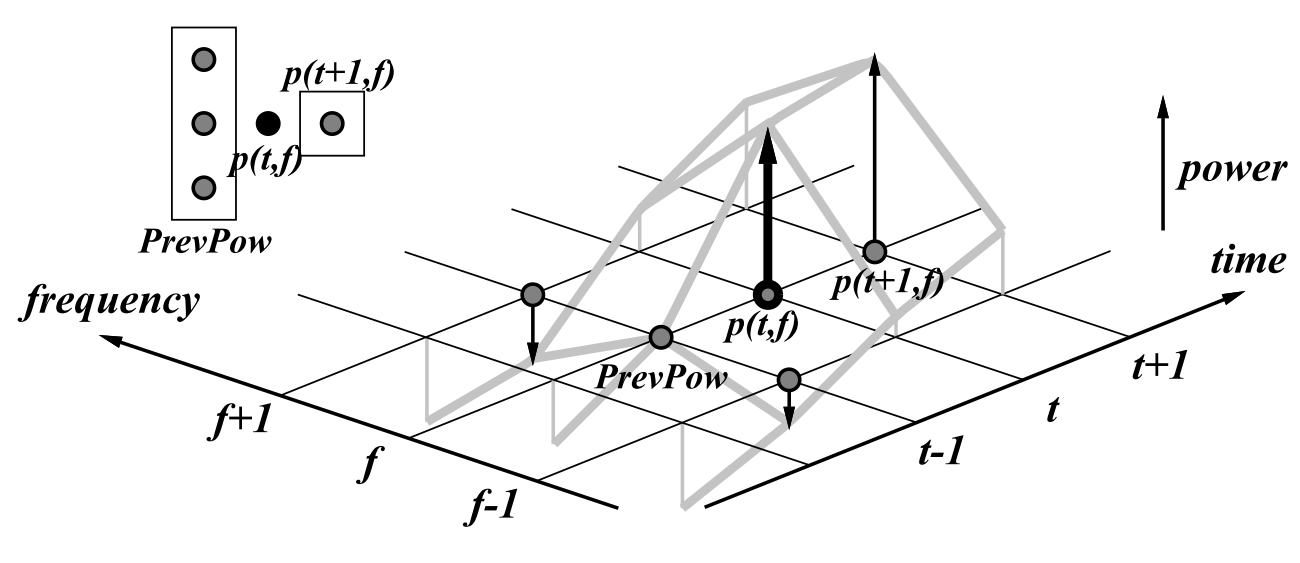
\includegraphics[scale=.25]{goto_onset}
                            \end{figure}
                        }
                    \end{itemize}
            \end{enumerate}
        \end{frame}
        \begin{frame}{onset detection}{novelty function: variants}
            \begin{itemize}
                \item	\textbf{number of frequency bands}
                    \begin{itemize}
                        \item	varies: 1, 3, 6, 21, 960, FFT length, ...
                        \item<2->	larger number of bands not necessarily better\\ $\rightarrow$ adjust number of band adaptively?
                    \end{itemize}
                \bigskip
                \item<3->	\textbf{combination of bands}
                    \begin{itemize}
                        \item	(weight and) add novelty functions per band
                        \item<4->	onset detection per band and combine results
                    \end{itemize}
            \end{itemize}
        \end{frame}
        \begin{frame}{onset detection}{peak picking: introduction}
            \vspace{-4mm}
            \begin{itemize}
                \item	detect onsets in the smoothed novelty function
                    \vspace{-5mm}
                    \figwithmatlab{NoveltyFunction}
                
                \item<2->	typical \textbf{criteria}
                    \begin{itemize}
                        \item<2->	local maximum \& salient peak
                        \item<3->	higher than minimum likelihood
                        \item<4->	not too close to maxima with higher likelihood
                        \item<5->	other options: high attack slope, distance to prev min, \ldots
                    \end{itemize}
            \end{itemize}
        \end{frame}
        \begin{frame}{onset detection}{peak picking: thresholding}
            \only<1-3>{
            \begin{itemize}
                \item fixed threshold
                \begin{equation*}
                    G_{d,\mathrm{c}} = \lambda_1 
                \end{equation*}
                \item<2->	smoothed threshold
                \begin{equation*}
                    G_{d,\mathrm{ma}} = \lambda_2 + \sum\limits_{j=0}^{\mathcal{O}-1}{b(j)\cdot d(i-j)}
                \end{equation*}
                \item<3->	median threshold
                \begin{equation*}
                    G_{d,\mathrm{me}} = \lambda_2 + \hat{Q}_d(0.5) 
                \end{equation*}
            \end{itemize}
            }
            \only<4>{
            \figwithmatlab{PeakPicking}
            }
        \end{frame}
        \begin{frame}{onset detection}{evaluation}
            \question{how do you properly evaluate an onset detection system}
            \begin{itemize}
                \item   methodology
                \smallskip
                \item   ground truth
                    \begin{itemize}
                        \item   how to get/generate
                        \item   necessary annotations
                    \end{itemize}
                \smallskip
                \item   metrics
                    \begin{itemize}
                        \item   how to measure the accuracy of your system
                    \end{itemize}
            \end{itemize}
        \end{frame}

    %%	\begin{frame}{onset detection}{evaluation: introduction}
    %%	\end{frame}
    %%	\begin{frame}{onset detection}{evaluation: metrics}
    %%	\end{frame}
    %%	\begin{frame}{onset detection}{evaluation: test data set}
    %%	\end{frame}
    %
    \section[tempo]{beat \& tempo detection}
        \begin{frame}{tempo detection}{brainstorm}
            \question{what are your ideas for detecting the tempo and the beats in a complex mixture}
        \end{frame}
        \begin{frame}{tempo detection and beat tracking}{introduction}
            \begin{itemize}
                \item \textbf{objectives}
                    \begin{enumerate}
                        \item	find the tempo from the novelty function/onsets
                        \item	find the beat locations
                    \end{enumerate}
                \bigskip
                \item<2-> \textbf{systematic problems}:
                    \begin{enumerate}
                        \item	distinguish \textit{hierarchical levels}
                            \begin{itemize}
                                \item[]	
                                \item	meter
                                \item	beat
                                \item	subbeat/tatum
                            \end{itemize}
                            \vspace{-17mm}
                            \begin{flushright}
                                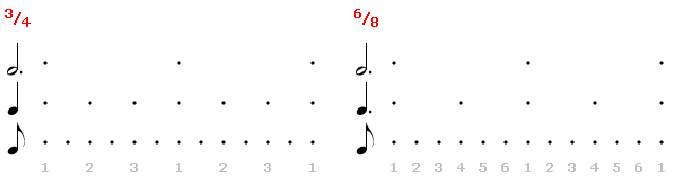
\includegraphics[scale=.25]{graph/periodiclevels}
                            \end{flushright}
                        \item<3->	detect \textit{beats without onsets}
                        \item<3->	recognize \textit{onsets without beats}
                    \end{enumerate}
            \end{itemize}
            
        \end{frame}
        \begin{frame}{tempo detection and beat tracking}{oscillator approach}
            \textbf{Beat tracking with an oscillator}\footfullcite{large_beat_1995}
            \begin{figure}
                \centering
                    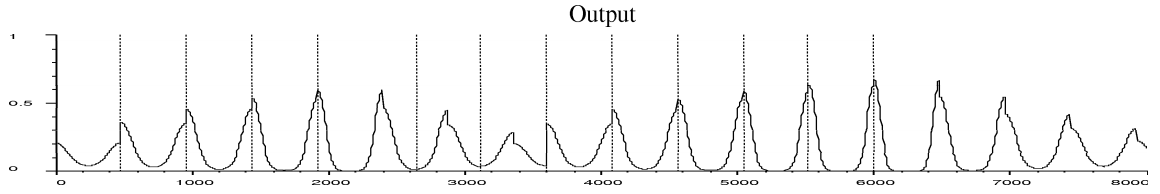
\includegraphics[scale=.3]{graph/BPM_large_oscillator}
            \end{figure}
            
            \begin{enumerate}
                \item	initialize pulse generator (tempo estimate, beat position estimate)
                \item<2->	predict next beat location with pulse
                \item<3->	adapt acc.\ to distance (predicted vs.\ real onset position)
                    \begin{itemize}
                        \item	beat period
                        \item	beat phase
                    \end{itemize}
                \item<4->	predict with adapted settings
                \item<4->   adapt \ldots
            \end{enumerate}
        \end{frame}
        \begin{frame}{tempo detection and beat tracking}{oscillator approach: initialization}
            \question{How to estimate the initial tempo}

            \begin{itemize}
                \item	location of maximum of \textbf{ACF of novelty function}
                \item<2->	maximum of \textbf{IOI histogram}
                    \begin{figure}
                        \centering
                            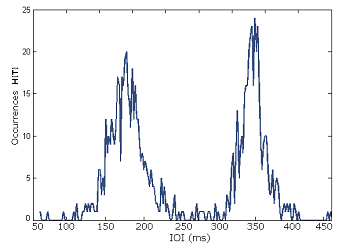
\includegraphics[scale=.3]{graph/ioi_hist}
                    \end{figure}
                \item<3->	maximum of \textbf{beat spectrum/histogram}
                \item<3->	\ldots
            \end{itemize}
        \end{frame}
        \begin{frame}{tempo detection and beat tracking}{multi-agent approach}
            \begin{enumerate}
                \item	run \textbf{multiple beat trackers} with different parameters
                    \begin{itemize}
                        \item	initial tempo
                        \item	initial beat phase
                        \item	adaptation speed
                    \end{itemize}
                \item<2->	compute reliability/confidence criteria:
                
                    \begin{itemize}
                        \item	match beat and onset times
                        \item<3->	tempo stability
                        \item<4->	majority of different agents
                        \item   \ldots
                    \end{itemize}
                \item<5->	choose\textbf{ most reliable agent} (or path between agents)
            \end{enumerate}
        \end{frame}
        \begin{frame}{tempo detection and beat tracking}{filterbank approach}
            published by Scheirer\footfullcite{scheirer_tempo_1998}
            \begin{columns}[T]
            \column{.5\linewidth}
                \begin{enumerate}
                    \item	design \textbf{filterbank} (e.g. comb resonators spaced 1 beat)
                    \item<2->	compute filter output energy	
                    \item<3->	pick maximum
                \end{enumerate}
            \column{.5\linewidth}
                \only<1>{
                \begin{figure}
                    \centering
                        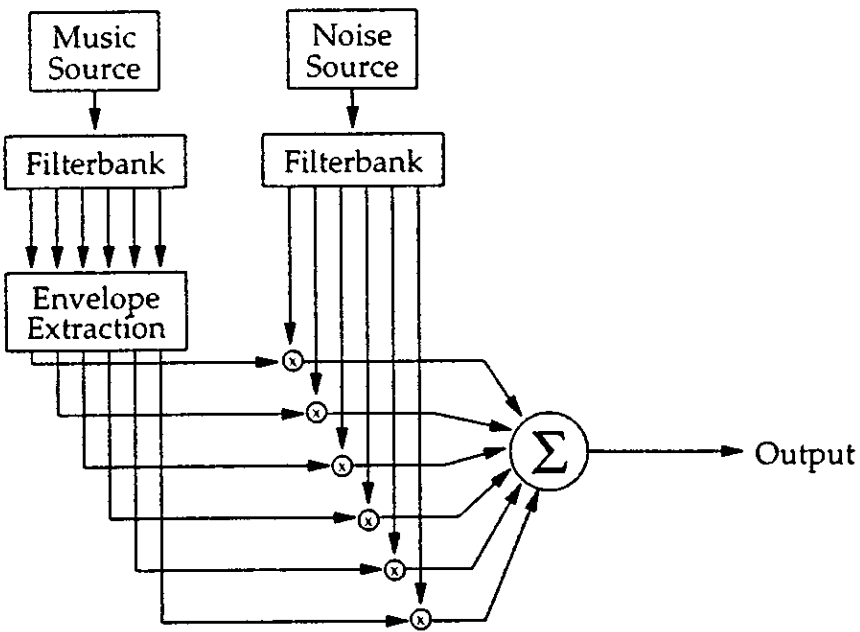
\includegraphics[scale=.25]{graph/BPM_Scheirer_filterbank}
                \end{figure}
                }
                \only<2>{
                \begin{figure}
                    \centering
                        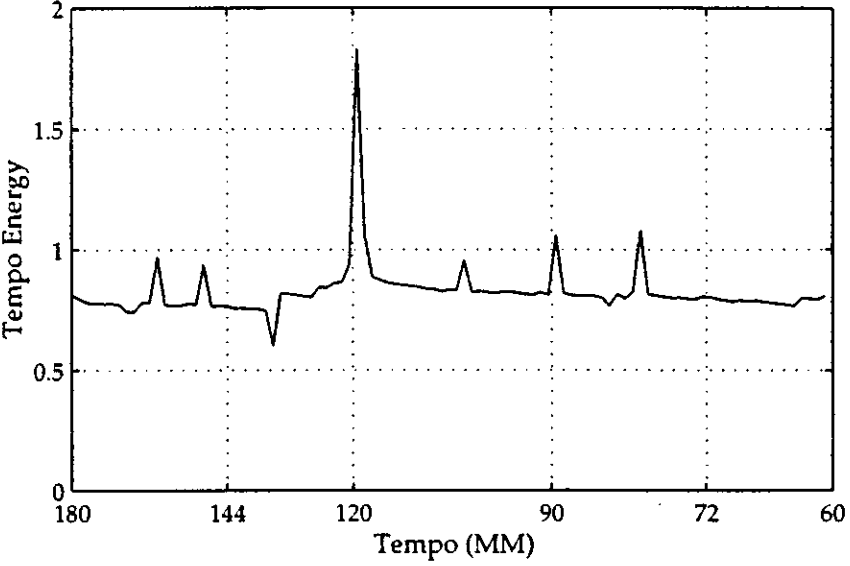
\includegraphics[scale=.25]{graph/BPM_Scheirer_beatspectrum}
                \end{figure}
                }
            \end{columns}
        \end{frame}
        \begin{frame}{tempo detection and beat tracking}{template-based approach}
            \begin{enumerate}
                \item	define set of \textbf{template pulses} in all tempi
                \item<2->	compute CCF between novelty function (or its ACF) and all templates
                \item<3->	choose template with highest correlation as tempo
                \item<4->	choose lag with highest correlation as beat phase
            \end{enumerate}
        \end{frame}
        \begin{frame}{tempo detection and beat tracking}{typical problems}
            \begin{enumerate}
                \item	tempo: detection of \textbf{double/half tempo} (triple, \ldots)
                \smallskip
                \item<2->	phase: detection of \textbf{off-beats}
                \smallskip
                \item<3->	tempo \& phase: strongly depends on \textbf{initialization values}
                \smallskip
                \item<4->	tempo \& phase: only \textbf{slow adaptation} --- no sudden tempo changes
                
                    \includeaudio{sonata-ck330_auftakt}
            \end{enumerate}
        \end{frame}
        \begin{frame}{tempo detection and beat tracking}{evaluation}
            \question{how do you properly evaluate a tempo detection or beat tracking system}
            \begin{itemize}
                \item   methodology
                \smallskip
                \item   ground truth
                    \begin{itemize}
                        \item   how to get/generate
                        \item   necessary annotations
                    \end{itemize}
                \smallskip
                \item   metrics
                    \begin{itemize}
                        \item   how to measure the accuracy of your system
                    \end{itemize}
            \end{itemize}
        \end{frame}

        \section[summary]{lecture summary}
        \begin{frame}{summary}{lecture content}
            \begin{enumerate}
                \item   why has so little work been done on the detection of \textit{offsets} (as opposed to onsets)
                \smallskip
                \item<2->   what is the difference between an onset and a beat
                \smallskip
                \item<3->   what are typical processing steps in an onset detection system --- describe approaches for each step
                \smallskip
                \item<4->   explain the terms tempo detection and beat tracking
                \smallskip
                \item<5->   describe basic approaches to tempo detection
            \end{enumerate}
        \end{frame}
\end{document}

